\documentclass[10pt, xcolor=table]{beamer}
\usepackage{inputenc}
\usepackage{graphicx}
\usepackage {mathtools}
\usetheme{CambridgeUS}
\usecolortheme{dolphin}
\usepackage{booktabs}
\usepackage{lscape}
\usepackage{caption}
\usepackage{tikz}
\usepackage{subcaption}
\usepackage{multicol}
\usepackage{xcolor}
\usepackage{pgfplots}
\usepackage{bm}
\usepackage{multicol}
\usepackage{adjustbox}
\usepackage{multicol}
\usepackage{cleveref}
\usepackage{tcolorbox}
\usepackage{changepage}
\usepackage{pifont}    % For more symbols like dingbats
\usepackage{blindtext}
\usepackage{array}
\usepackage{diagbox}

\newcommand\dc[1]{\textcolor{blue}{#1}}
\setcounter{tocdepth}{3}
\pgfplotsset{compat=1.16}
%\usetikzlibrary{external}
%\tikzexternalize[prefix=images/]

\newlength\figureheight
\newlength\figurewidth

\definecolor{myNewColorA}{HTML}{952748}
\definecolor{myNewColorB}{HTML}{ffe7ee} 
\definecolor{myNewColorC}{HTML}{c86666}
\definecolor{myNewColorD}{HTML}{eaa1a1} 
\definecolor{background_color}{HTML}{000000}

\setbeamercolor*{palette primary}{bg=myNewColorC}
\setbeamercolor*{palette secondary}{bg=myNewColorB, fg=black}
\setbeamercolor*{palette tertiary}{bg=myNewColorA, fg=white}
\setbeamercolor*{titlelike}{fg=myNewColorA}
\setbeamercolor*{title}{bg=myNewColorA, fg=white}
\setbeamercolor*{item}{fg=myNewColorB}
\setbeamercolor*{caption name}{fg=myNewColorA}

% For NN graph

\usepackage{listofitems} % for \readlist to create arrays
\usetikzlibrary{arrows.meta} % for arrow size
\usepackage[outline]{contour} % glow around text
\contourlength{1.4pt}


% STYLES
\tikzset{
	>=latex, % for default LaTeX arrow head
	node/.style={thick,circle,draw=myblue,minimum size=22,inner sep=0.5,outer sep=0.6},
	node in/.style={node,green!20!black,draw=mygreen!30!black,fill=mygreen!25},
	node hidden/.style={node,blue!20!black,draw=myblue!30!black,fill=myblue!20},
	node convol/.style={node,orange!20!black,draw=myorange!30!black,fill=myorange!20},
	node out/.style={node,red!20!black,draw=myred!30!black,fill=myred!20},
	connect/.style={thick,mydarkblue}, %,line cap=round
	connect arrow/.style={-{Latex[length=4,width=3.5]},thick,mydarkblue,shorten <=0.5,shorten >=1},
	node 1/.style={node in}, % node styles, numbered for easy mapping with \nstyle
	node 2/.style={node hidden},
	node 3/.style={node out}
}
\def\nstyle{int(\lay<\Nnodlen?min(2,\lay):3)} % map layer number onto 1, 2, or 3

\usefonttheme{professionalfonts}



%\usepackage[round]{natbib} % or use 'authoryear' if you prefer
%\usepackage{natbib}
\usepackage{hyperref}
%------------------------------------------------------------
\titlegraphic{
	\begin{figure}
		\centering
		\begin{subfigure}[l]{0.45\textwidth}
			\centering
			
\includegraphics[width=2.5cm,height=1.5cm]{./Logo_U.T.P.png}
		\end{subfigure}
		\hfill
		\begin{subfigure}[r]{0.45\textwidth}
			\centering
			
\includegraphics[width=2.5cm,height=2.5cm]{./logo-maestria-scaled.jpg}
		\end{subfigure}
	\end{figure}
}

\setbeamerfont{title}{size=\Large\bfseries}
\setbeamerfont{subtitle}{size=\footnotesize}
\setbeamerfont{author}{size=\small}
\setbeamerfont{institute}{size=\footnotesize}

\title[Universidad Tecnológica de Pereira]{Data-Driven Models for Identifying Mental Disorders in Students and Enhancing Therapy Scheduling}



\author[Julián David Pastrana-Cortés]{%
	\texorpdfstring{
		\begin{tabular}{c}
			M.Sc. Julián David Pastrana-Cortés \\[1.5mm]
%			\textbf{Director}: Álvaro Angel Orozco-Gutiérrez \\[1.5mm]
%			\textbf{Co-director}: David Augusto Cardenas-Peña
		\end{tabular}
	}{Julián David Pastrana-Cortés\vspace{-20pt}}
}

\institute[Automatics]{Automatics Research Group\vspace{-15pt}}
%\date{\today\vspace{-15pt}}

\AtBeginSection[]{
	\begin{frame}
		\vfill
		\centering
		\begin{beamercolorbox}[sep=8pt,center,shadow=true,rounded=true]{title}
			\usebeamerfont{title}\insertsectionhead\par%
		\end{beamercolorbox}
		\vfill
	\end{frame}
}

\usepackage{ragged2e} % For \justifying command
\usepackage{lipsum} % Only for demo text

\addtobeamertemplate{block begin}{}{\justifying} 
%\addtobeamertemplate{itemize begin}{}{\justifying} 


%------------------------------------------------------------

\usepackage{etoolbox}

\apptocmd{\frame}{}{\justifying}{} 
\let\olditem\item
\renewcommand\item{\olditem\justifying}

\begin{document}
	
\frame{\titlepage}



\section*{Mental Disorders}

\begin{frame}{Understanding Mental Disorders}
	A mental disorder refers to a significant disturbance in an individual's cognition, emotional regulation, or behavior.
	
	\begin{multicols}{2}
		
		\begin{figure}[t]
			\centering
			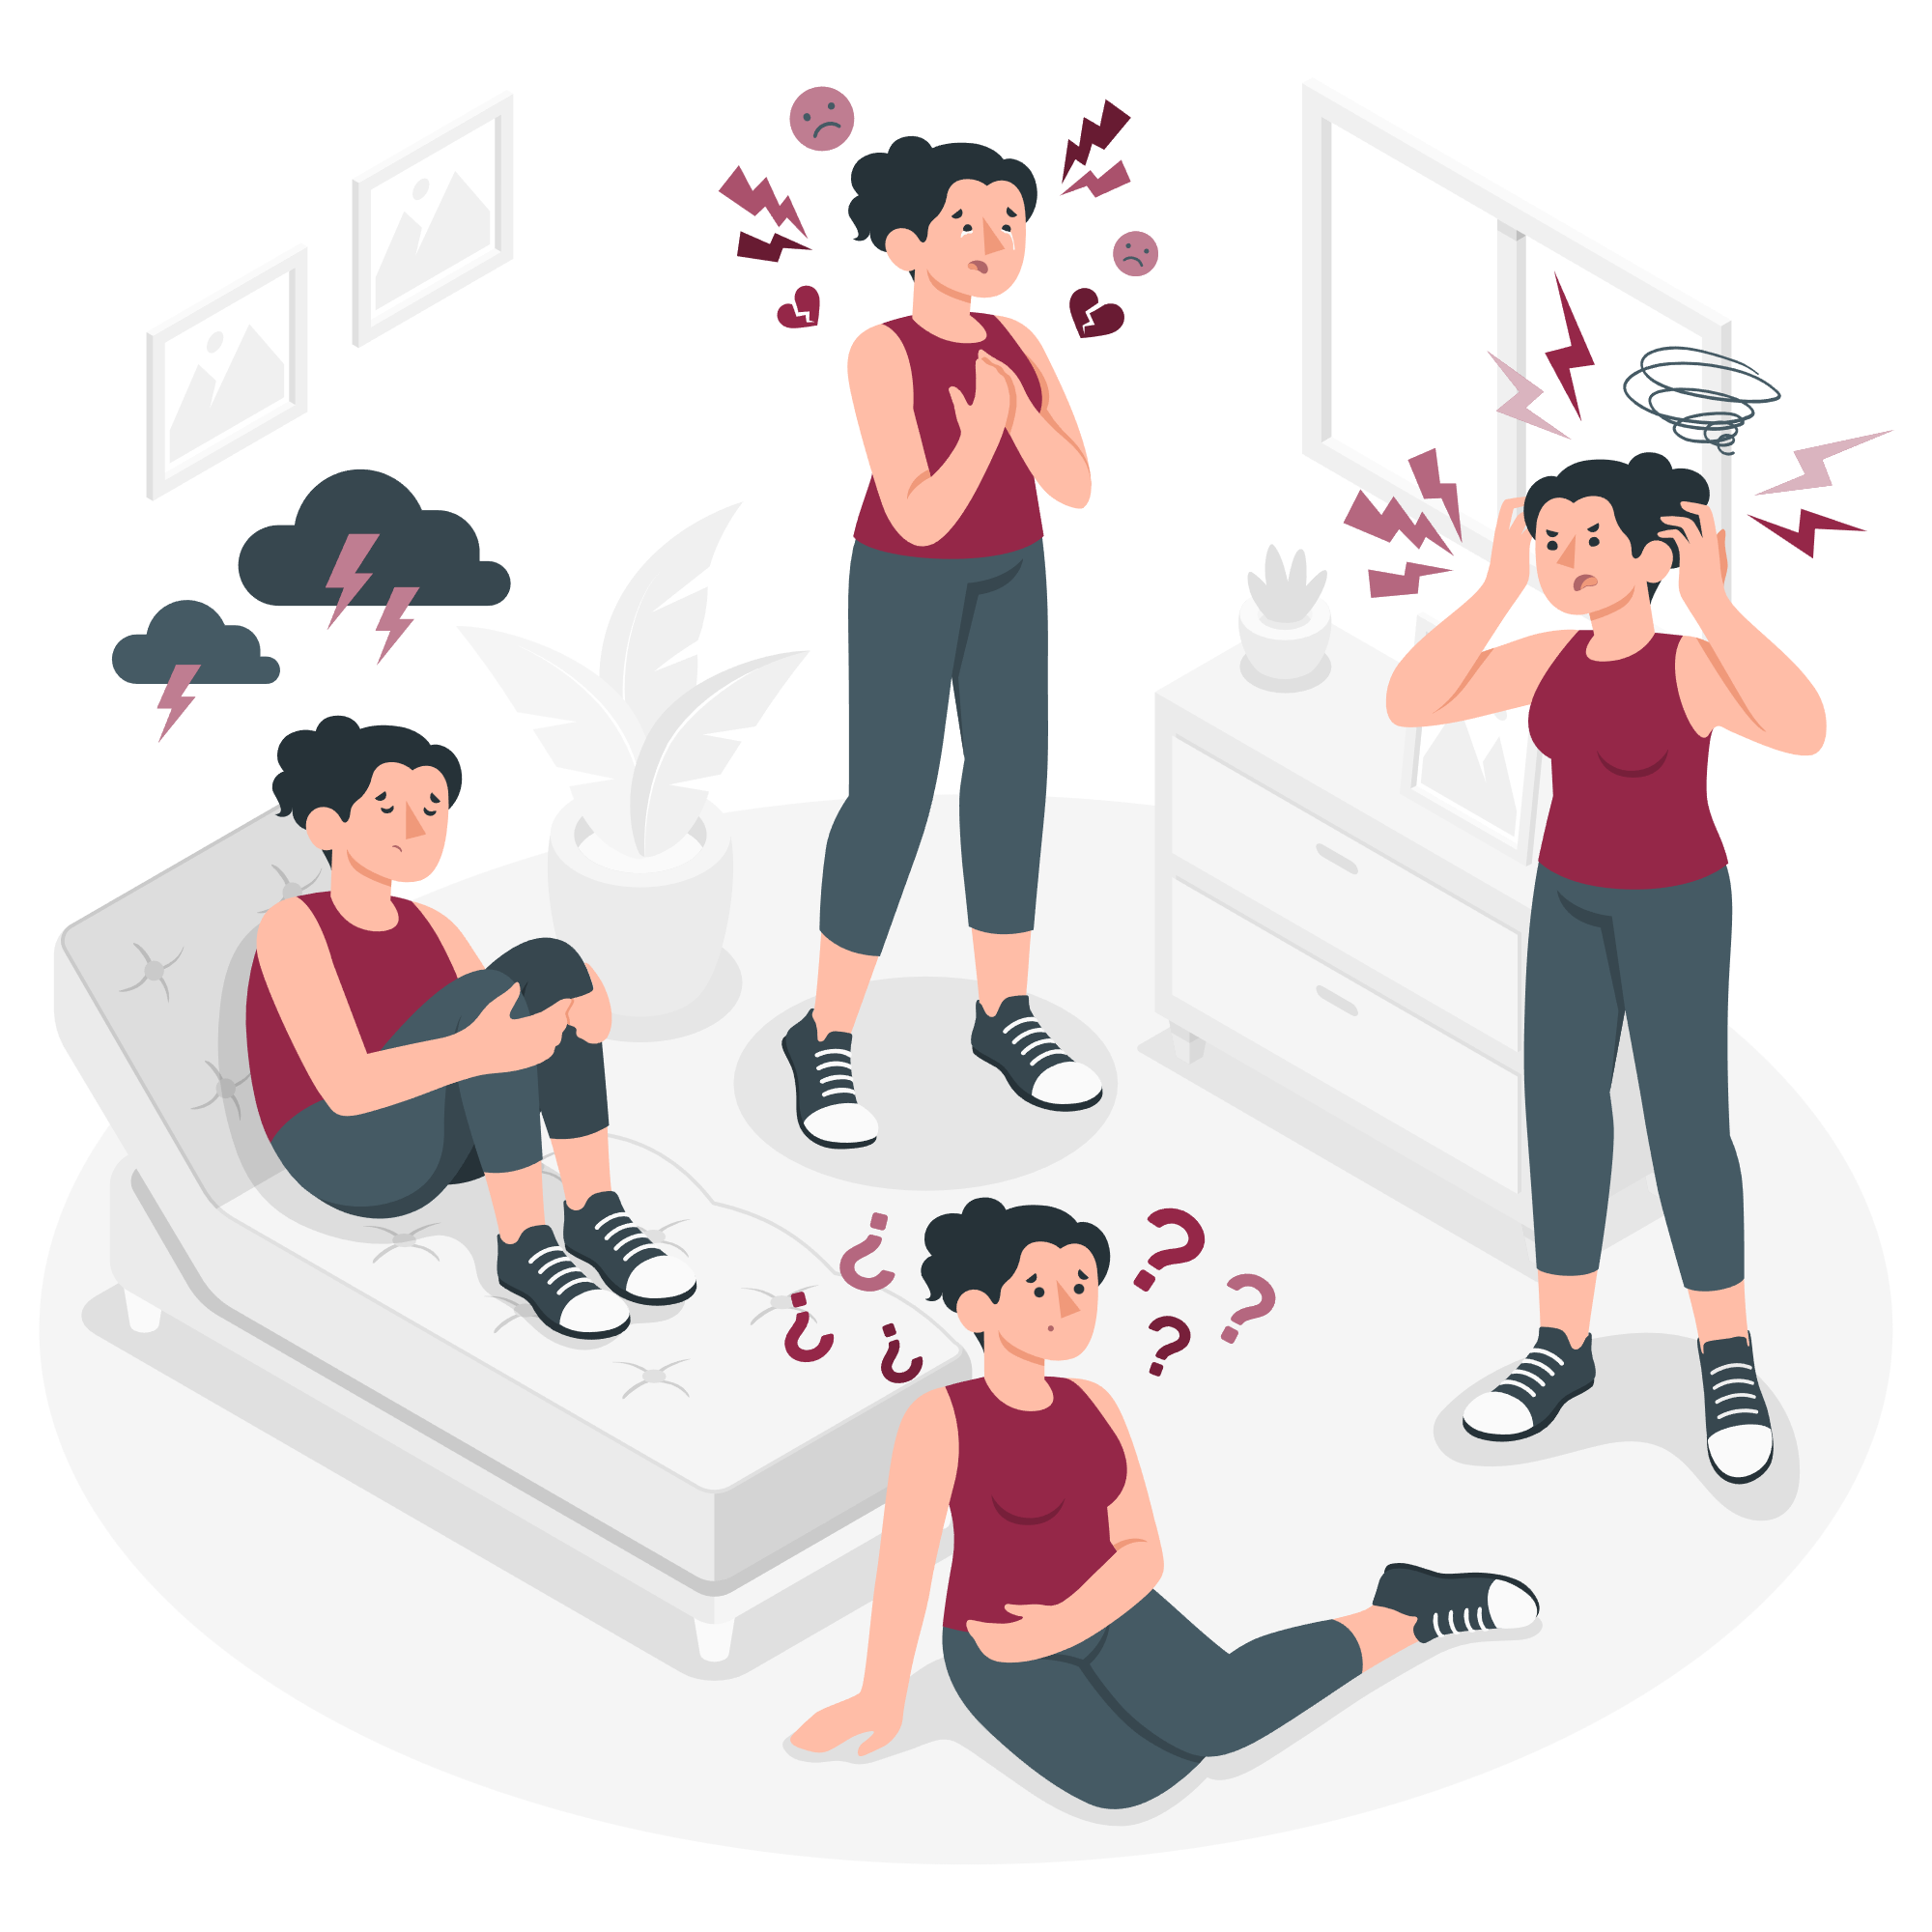
\includegraphics[width=0.8\linewidth]{./figures/mental_disorders.png}
		\end{figure}
		
		\columnbreak
		
		\vfill
		\begin{center}
			\begin{itemize}
				\item \textbf{Depression}: Persistent feelings of sadness and loss of interest.
				\item \textbf{Anxiety}: Excessive fear or worry, often irrational.
				\item \textbf{Impulsivity}: Acting without thought or consideration of consequences.
				\item \textbf{Hyperactivity}: Excessive movement, often interfering with daily activities.
			\end{itemize}
		\end{center}
		
		\vfill
		
	\end{multicols}
	
	Over 350 million individuals worldwide suffer from mental disorders \cite{DEHGHANBONARI2023100238}.
	
\end{frame}


\begin{frame}{Why Accurate Diagnosis Matters for Students?}
	\begin{columns}
		\begin{column}{0.5\textwidth}
			\begin{itemize}
				\item Mental health disorders can significantly impact students' academic and social lives \cite{HAMORI2023115139}.
				\item External factors, such as homesickness and family expectations, can intensify mental health issues \cite{DEHGHANBONARI2023100238}.
				\item Anxiety and depression, the most common mental health concerns among U.S. college students, have been on the rise \cite{https://doi.org/10.1002/jcad.12543}.
				\item There is a lack of effective tools to identify at-risk students before issues escalate \cite{HAMORI2023115139}.
			\end{itemize}
		\end{column}
		\begin{column}{0.5\textwidth}
			\begin{figure}[t]
				\centering
				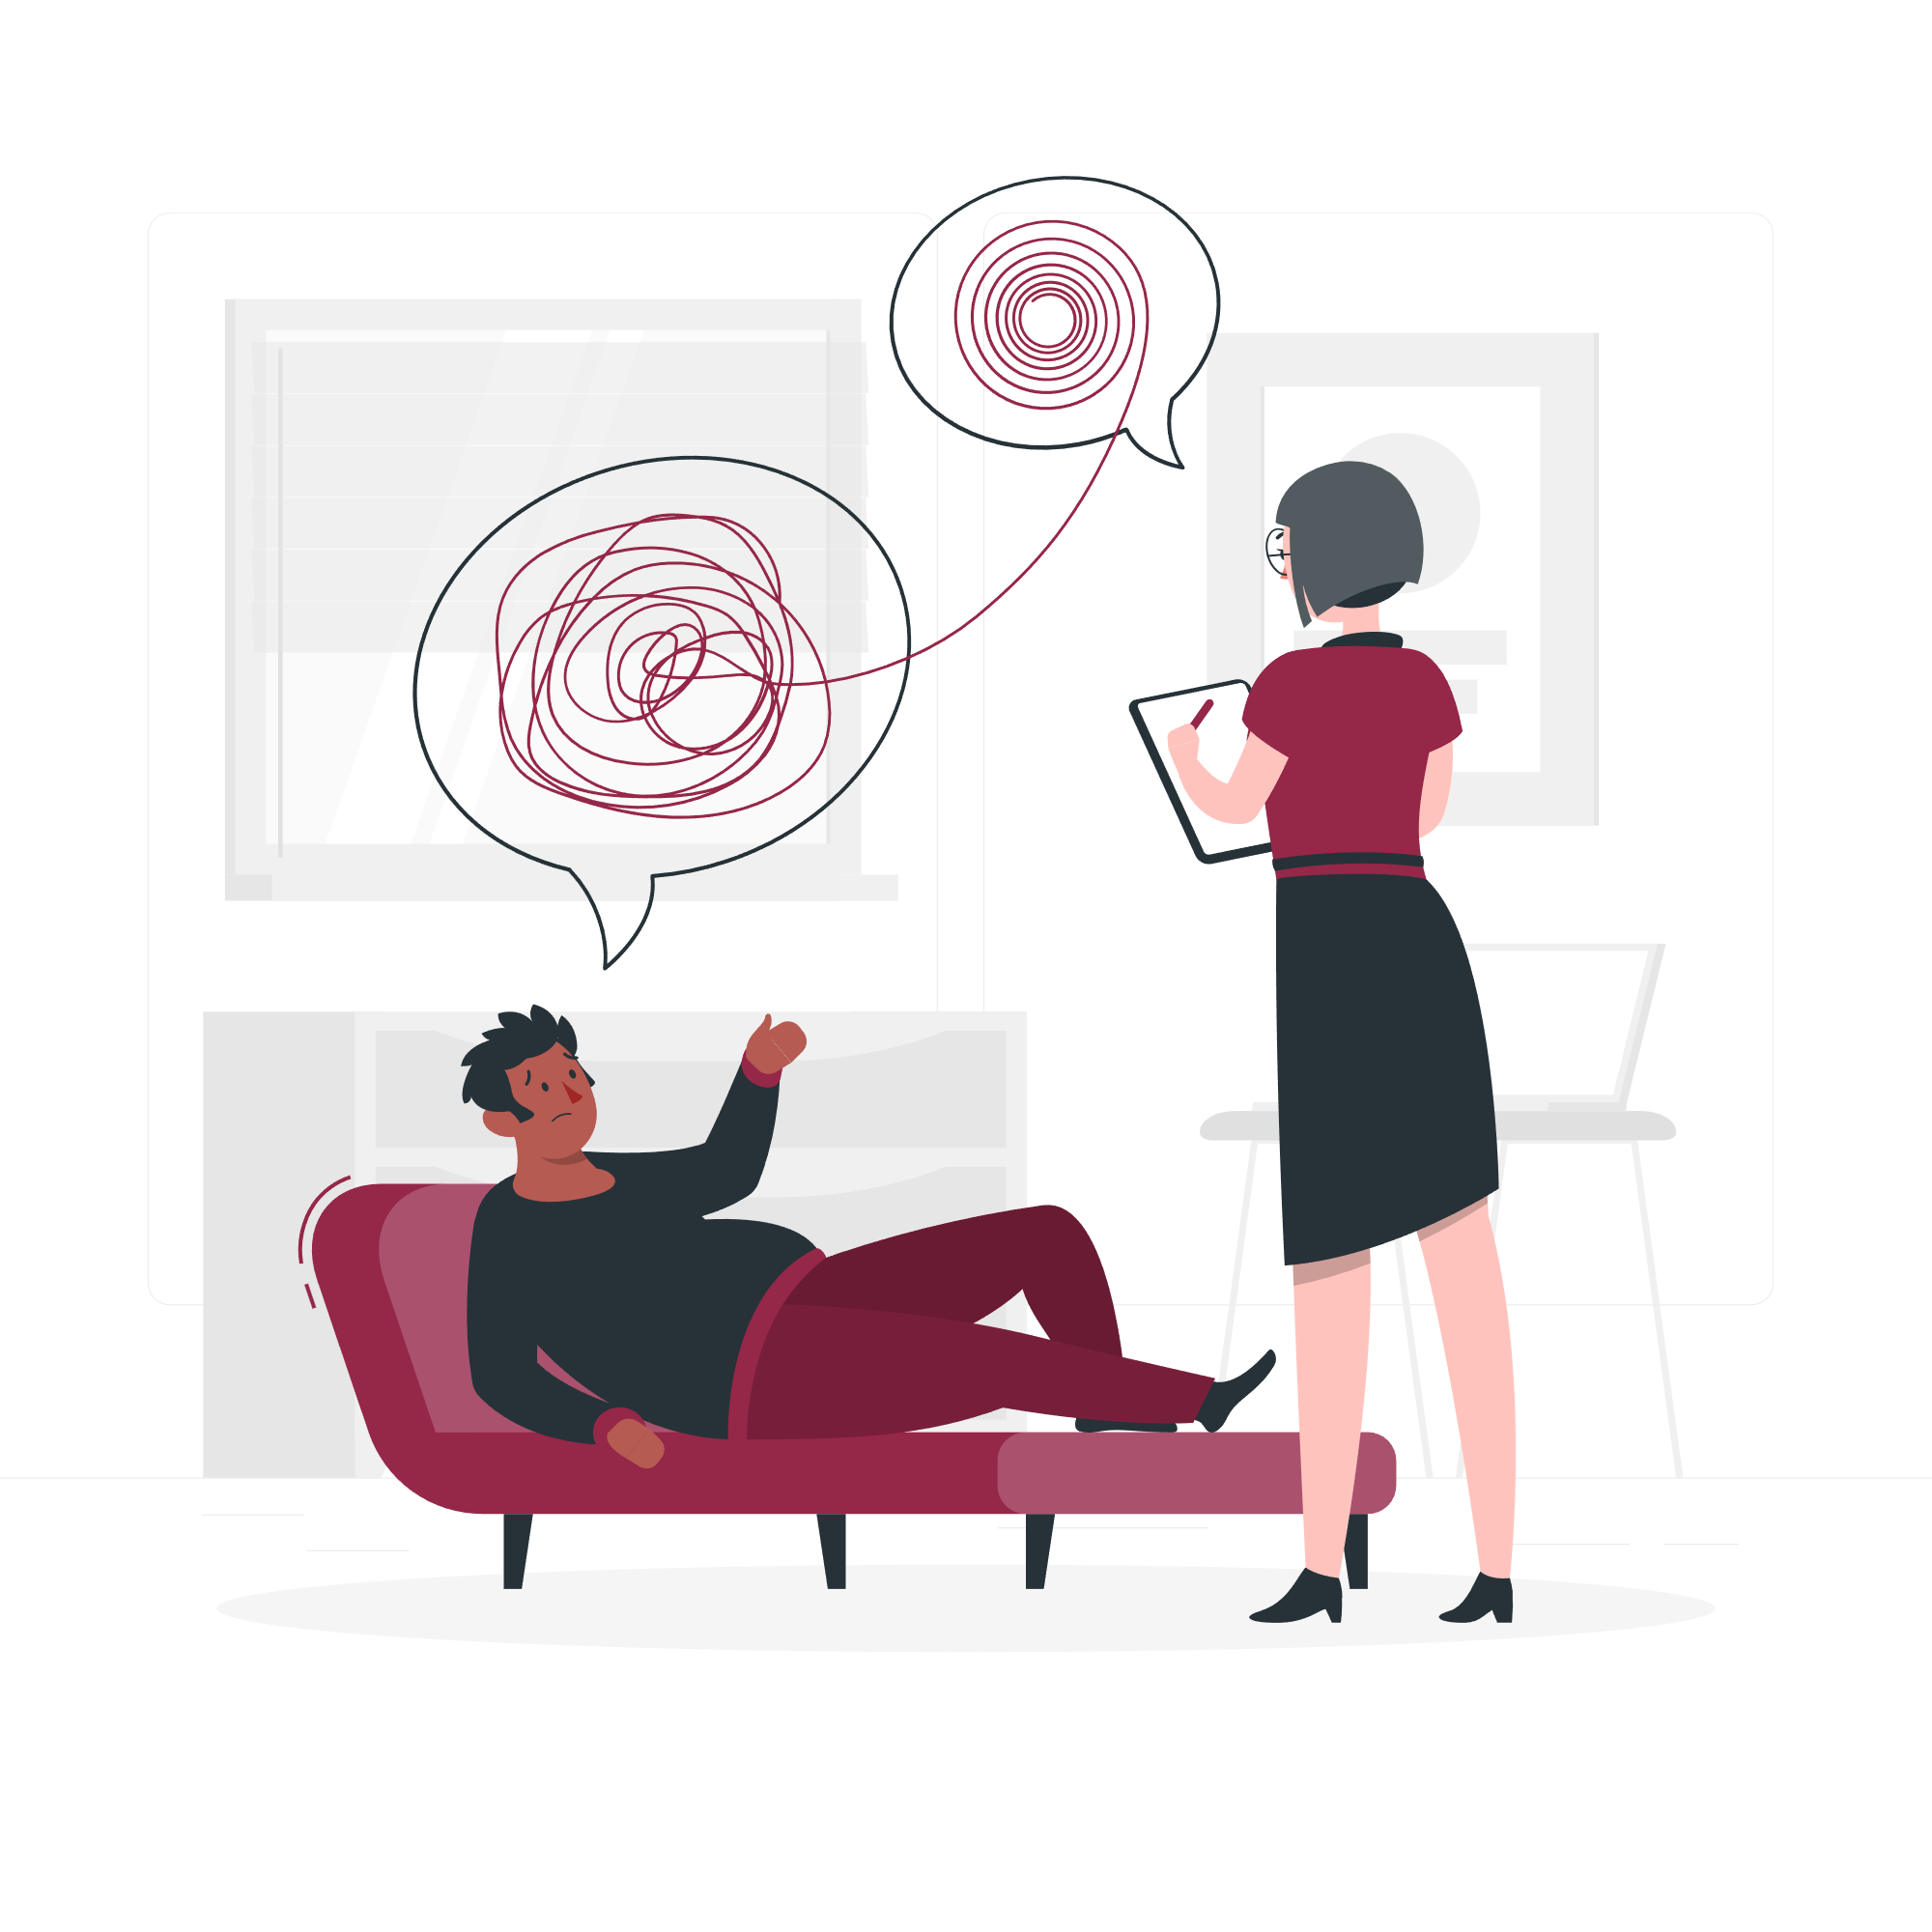
\includegraphics[width=\linewidth]{./figures/psychologist.png}
			\end{figure}
		\end{column}
	\end{columns}
\end{frame}

\section*{Data-Driven Models}

\begin{frame}{Data-Driven Models}

	As the ability to collect and process data has advanced, leveraging evidence to identify patterns is now essential for supporting accurate diagnoses and planning effective therapies.
	
	\vspace{-1.5cm}
	
	\begin{figure}
	\centering
	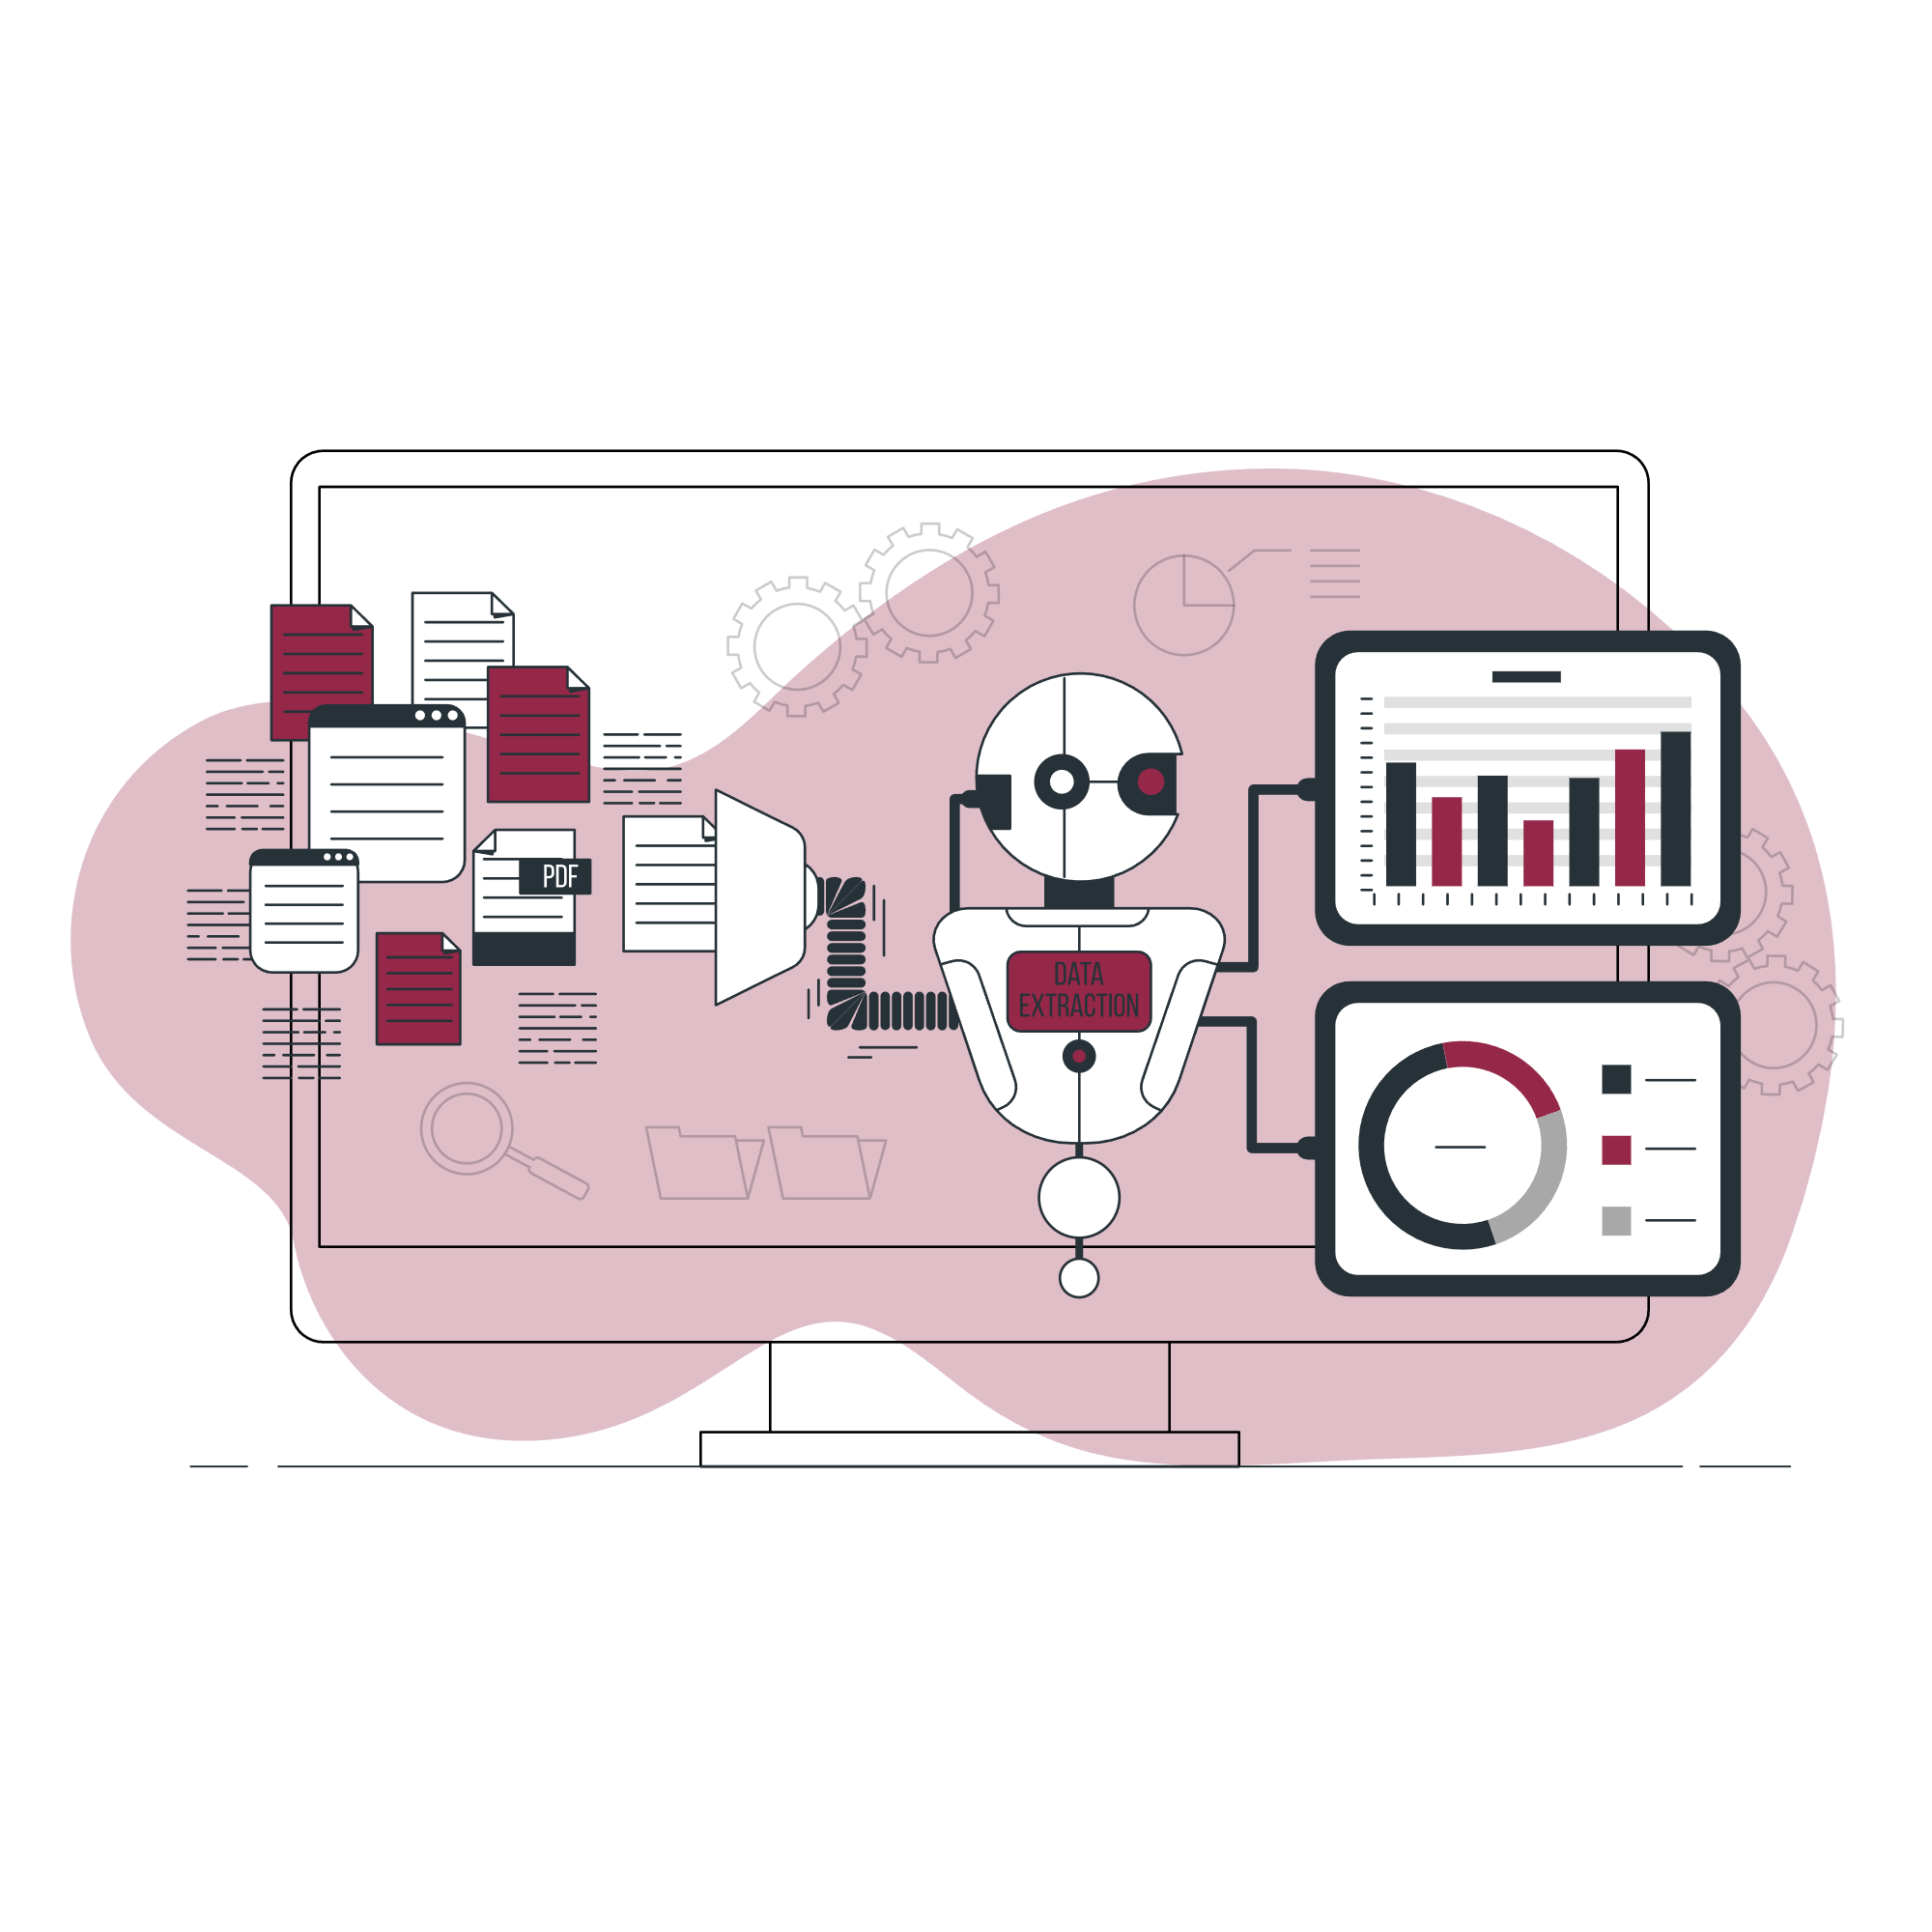
\includegraphics[width=0.6\linewidth]{./figures/data_driven.png}
	\end{figure}		
	
	\vspace{-1.5cm}
	A question arises: Why shouldn't schools use data-driven methods to identify mentally ill students? \cite{DEHGHANBONARI2023100238}
\end{frame}

\begin{frame}{Machine Learning Models}
	\begin{columns}[T]
		\begin{column}{0.5\textwidth}
			\justifying
			While machine learning models, as a subset of data-driven models, are designed to adapt to complex phenomena without explicit programming.
			
			\vspace{0.5cm}
			Machine learning models continuously learn and refine their predictions as more data becomes available.
		\end{column}
		\begin{column}{0.5\textwidth}
			\centering
			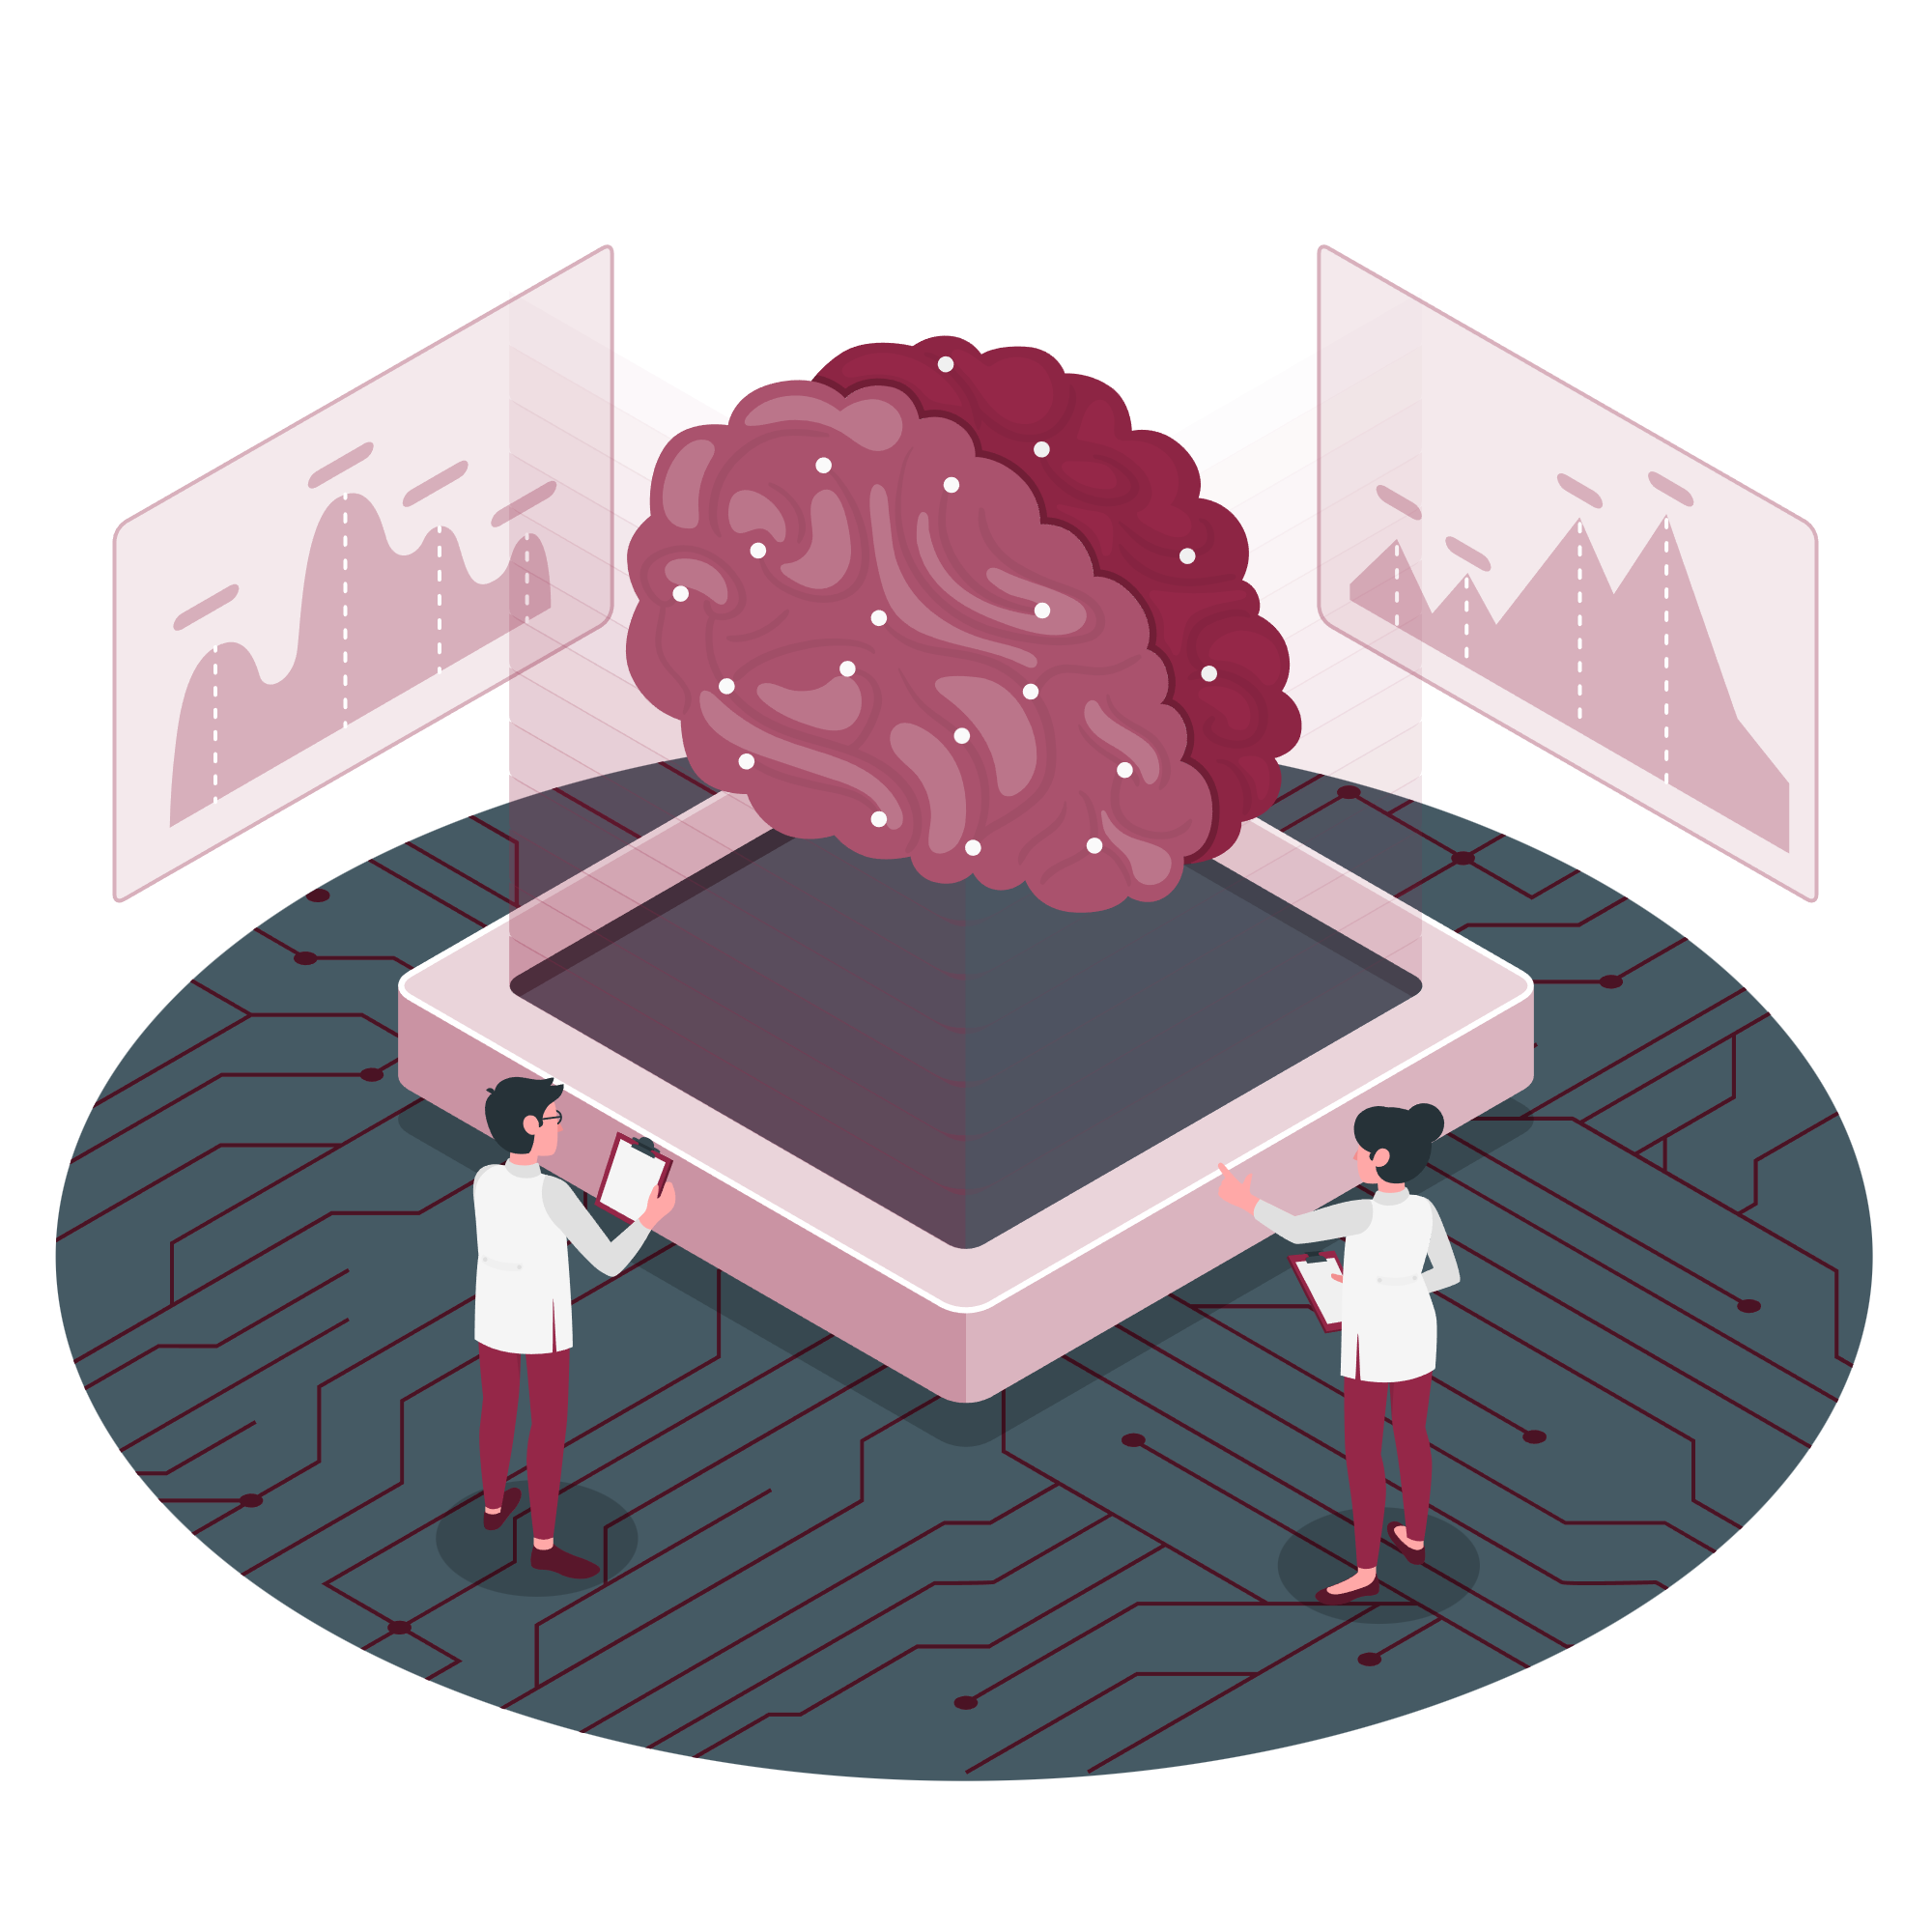
\includegraphics[width=\linewidth]{./figures/artificial_intelligence.png}
		\end{column}
	\end{columns}
\end{frame}


\begin{frame}{The Role of Machine Learning in Mental Health Counseling}
	
	\justifying
	Machine learning models are not a replacement for professional counselors but a tool to enhance their work. These models:
	\begin{itemize}
		\item Provide a data-informed foundation for developing prevention and intervention strategies.
		\item Identify students at heightened risk of mental health disorders such as anxiety and depression.
		\item Reduce demands on time, manpower, and resources while maintaining effectiveness.
		\item Highlight features that contribute to mental health predictions.
	\end{itemize}
	
	
\end{frame}


\section*{Methodology}

\begin{frame}{Three-Step Module-Based Methodology}

	
	\vspace{0.5cm}
	
	\begin{columns}[c]
		\column{0.33\textwidth}
		\centering
		\textbf{Mental Disorder Identification} \\
		
\includegraphics[width=\linewidth]{./figures/identification.png}
		
		\column{0.33\textwidth}
		\centering
		\textbf{Student Prioritization} \\
		
\includegraphics[width=\linewidth]{./figures/priorizing.png}
		
		\column{0.33\textwidth}
		\centering
		\textbf{Therapy scheduling} \\
		
\includegraphics[width=\linewidth]{./figures/schedule.png}
	\end{columns}
\end{frame}

\section*{Mental Disorder Identification}

\begin{frame}{Data Collection and Labeling}
	
	\begin{columns}[c]
		\column{0.5\textwidth}
		\centering
		Data Collection \\
		\vspace{0.3cm}
		\begin{tcolorbox}[width=\linewidth, colback=myNewColorB, colframe=myNewColorA, boxrule=0.7mm, rounded corners]
			\justifying
			\begin{itemize}
				\item Emails, forms, messages
				\item Course-related groups
				\item Student affairs office data
				\item Supervision by psychiatrists
			\end{itemize}
		\end{tcolorbox}
		
		\column{0.5\textwidth}
		\centering
		Data Labeling \\
		\vspace{0.3cm}
		\begin{tcolorbox}[width=\linewidth, colback=myNewColorB, colframe=myNewColorA, boxrule=0.7mm, rounded corners]
			\justifying
			Expert labeling ensures reliable data for analysis, addressing cases with indirect or hard-to-measure target variables.
		\end{tcolorbox}
	\end{columns}
	
	\vspace{0.5cm}
	\centering
	\vspace{0.3cm}
	Input Space: \( \mathcal{X} \) (data features) \\
	Output Space: \( \mathcal{Y} = \{(l, s)\} \) \\
	\vspace{0.2cm}
	\begin{itemize}
		\item \( l \): Multi-label classification for different mental disorders.
		\item \( s \): Severity level of the disorder, ranging from 0 (none) to 1 (severe).
	\end{itemize}
	
\end{frame}




\begin{frame}{Mental Disorder Classification}
	
	\begin{columns}[c]
		\column{0.6\textwidth}
		\justifying

		\vspace{0.3cm}
		Labeled text data is used to train a machine learning model for mental disorder classification. The model classifies individuals as healthy or with mental disorders to aid diagnosis.
		
		\column{0.4\textwidth}
		\centering
		\vspace{-0.3cm}
		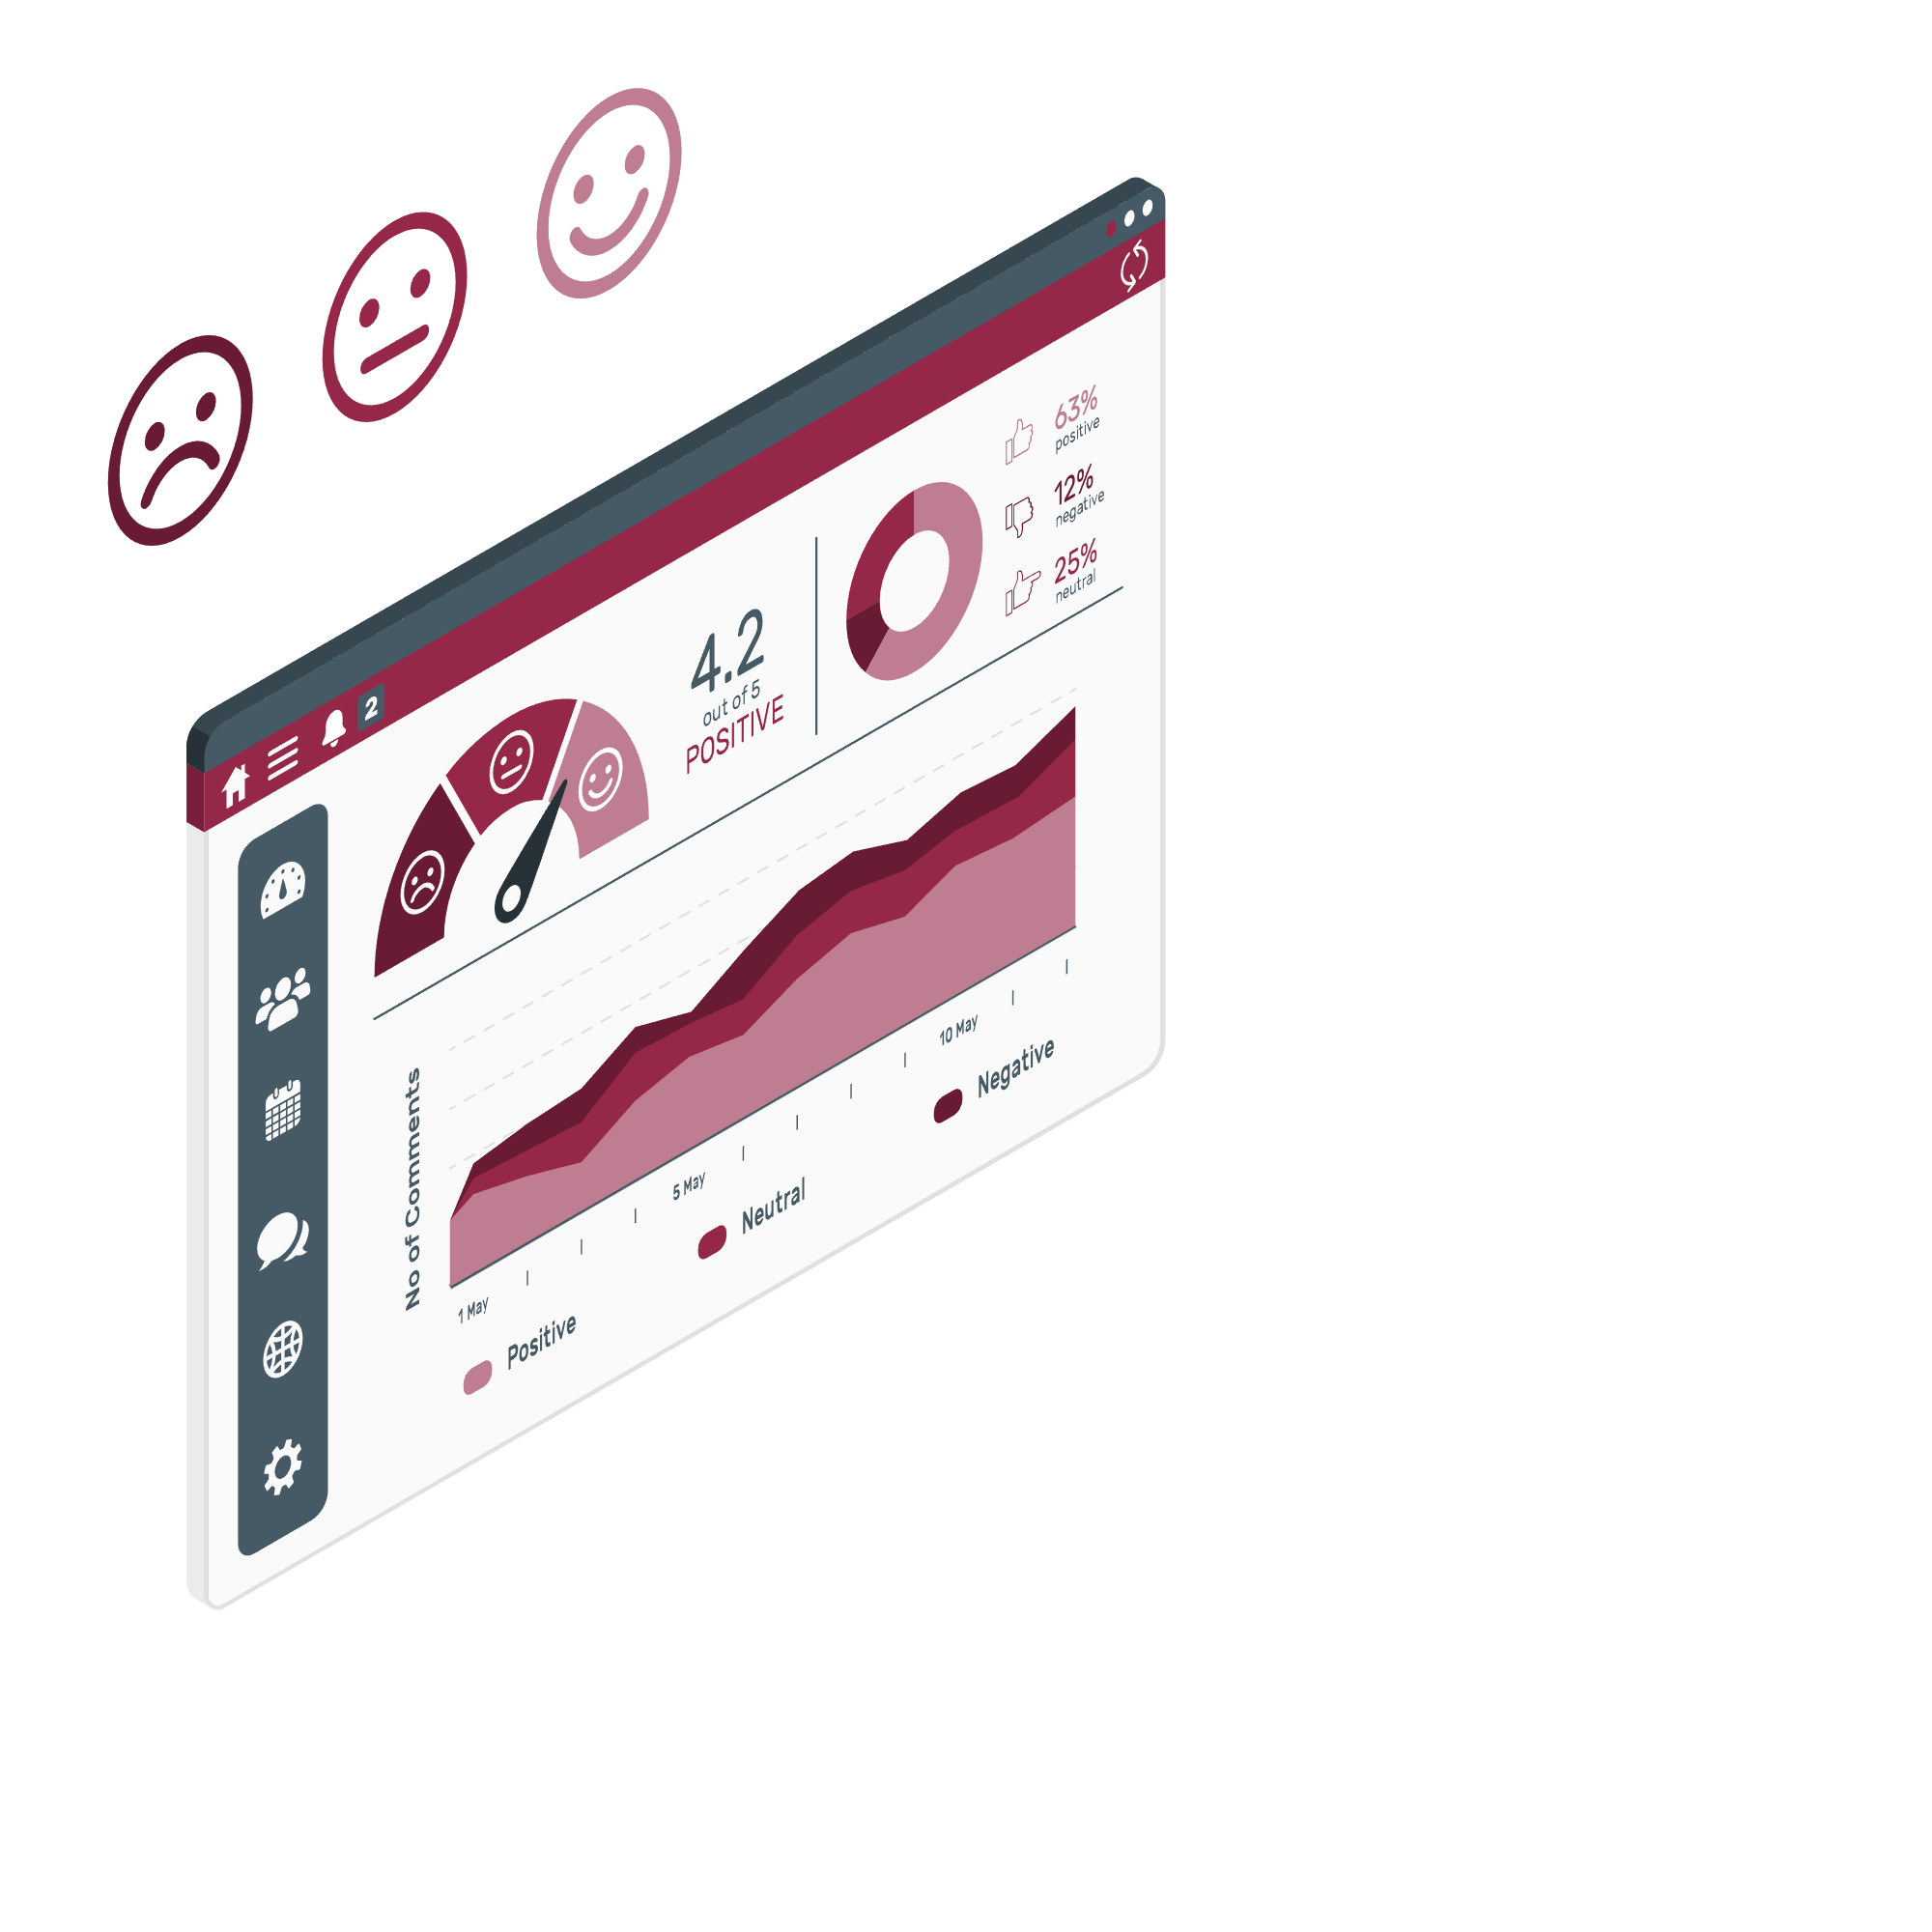
\includegraphics[width=\linewidth]{./figures/sentimental_analysis.png} % Replace with your actual image path
	\end{columns}
	
\end{frame}


\section*{Student Prioritization}

\begin{frame}{Prioritization of Students for Treatment}
	
	\begin{columns}[c]
		\column{0.6\textwidth}
		\justifying
		Using the same input space \( \mathcal{X}\), a model trained on severity levels \( s \in [0, 1] \) is applied. \\
		\vspace{0.3cm}
		This model prioritizes students based on the severity of their mental disorders, allowing for:
		\begin{itemize}
			\item Identification of students needing urgent psychological support.
			\item Optimization of resources by efficiently allocating psychological professionals.
			\item Ensuring timely and focused interventions for those with the highest severity levels.
		\end{itemize}
		
		\column{0.4\textwidth}
		\centering
		\vspace{-0.3cm}
		
\includegraphics[width=\linewidth]{./figures/priorizing.png}
	\end{columns}
	
\end{frame}


\begin{frame}{Scheduling Algorithms for Therapy Appointments}
	
	\centering
	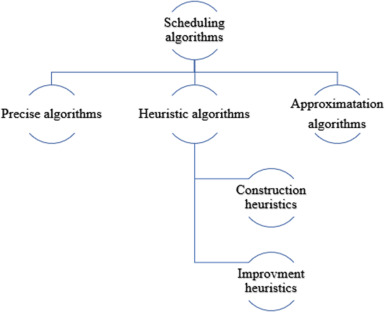
\includegraphics[width=0.65\linewidth]{./figures/scheduling_types.jpg} % Replace with your actual image path
	
\end{frame}


\section*{Case of Study}

\begin{frame}{Case of Study: A diagnostic analytics model for managing post-disaster symptoms of depression and anxiety among students using a novel data-driven optimization approach}
	
This study aims to implement and scrutinize a data-driven optimization method for identifying and providing therapy to students with symptoms of depression and anxiety.
\vspace{0.5cm}
	
	Findings:
\begin{itemize}
	\item Conventional methods detected only 7 to 15\% of cases.
	\item The proposed strategy improved detection rates to 44\%.
	\item Enhanced ability to identify and prioritize students for interventions.
\end{itemize}
	
\end{frame}

\begin{frame}{Case of Study: Machine learning predictive models to guide prevention and intervention allocation for anxiety and depressive disorders among college students}
	
	Machine learning models were used to identify US college students at heightened risk of diagnosable anxiety and depressive disorders.
	\vspace{0.5cm}
	
	Findings:
	\begin{itemize}
		\item Provides a proactive tool for counselors to identify at-risk students before conditions escalate.
		\item Offers data-driven insights to enhance understanding of mental health determinants.
		\item Guides prevention and intervention strategies to support diverse student populations.
		\item Promotes well-being through informed and targeted counseling approaches.
	\end{itemize}
	
\end{frame}

\section*{Final Remarks}

\begin{frame}{Conclusions}
	
	\begin{tcolorbox}[width=\textwidth, colback=myNewColorB, colframe=myNewColorA, boxrule=0.7mm, rounded corners]
		\begin{itemize}
			\item Increased identification accuracy of mental disorders compared to conventional methods.
			\item Prioritizes high-risk students using severity classification, optimizing therapy scheduling.
			\item Reduces waiting times and enhances access to mental health services.
			\item Supports informed decision-making by mental health professionals.
			\item Facilitates early-stage interventions, minimizing escalation of disorders.
		\end{itemize}
	\end{tcolorbox}
	
\end{frame}



\begin{frame}{Future Directions}
	
	\begin{tcolorbox}[width=\textwidth, colback=myNewColorB, colframe=myNewColorA, boxrule=0.7mm, rounded corners]
		\begin{itemize}
			\item Expand the methodology to include other mental health conditions.
			\item Explore integration with external mental health centers for advanced therapy options.
			\item Incorporate real-time monitoring systems to adapt models dynamically.
		\end{itemize}
	\end{tcolorbox}
	
\end{frame}



\bibliographystyle{plain}
\bibliography{refs}

	
\end{document}

952748

